% !TeX program = lualatex
% !TeX encoding = utf8
% !TeX spellcheck = uk_UA

\documentclass[]{beamer}


\usetheme{PlasmaPhysics}
\usepackage{PlasmaPhysics}
\newtcolorbox{mysidebyside}[1][]{
    notitle, sidebyside, blanker,
    sidebyside align=center seam,
    halign=center,
    lefthand width=.5\textwidth,
    #1
}
\graphicspath{{pictures/}}
\title[Лекції з фізики плазми]{\bfseries\huge Основні поняття}
\subtitle{\bfseries Лекції з фізики плазми}
\author{Пономаренко С. М.}
\date{}
% https://www.youtube.com/watch?v=zv9Y7YmHyBk
\def\stext#1{\text{
        \makebox[0pt]{
            \tikz[baseline] {\node[text width=50pt, align=center, execute at begin node=\setlength{\baselineskip}{-0.5ex}, blue] {#1};}
        }
}}




\title[Лекції з фізики плазми]{\bfseries\huge Основні поняття}
\author{Пономаренко С. М.}
\subtitle{Лекції з фізики плазми}
\date{}
\setbeamercovered{transparent=25}

\begin{document}
%=======================================================================================================
\usebackgroundtemplate{
	\tikz\node[opacity=0.1]{\includegraphics[width=\paperwidth,height=\paperheight]{background}};%
}


\begin{frame}
	\titlepage
\end{frame}

% ============================== Слайд ## ===================================
\begin{frame}{Що таке плазма?}{}
	\begin{block}{}
		\alert{Плазма} --- \emph{\alert{квазінейтральний}} газ заряджених частинок (частково або повністю іонізований газ).
	\end{block}

	\begin{block}{}\justifying\small
		Термін <<плазма>> в фізиці був уведений у 1923 американськими вченими І.Ленгмюром і Л.Тонксом, що робили зондові вимірювання параметрів низькотемпературної  газорозрядної  плазми.
	\end{block}

	\begin{block}{}
		За сьогоднішніми уявленнями $99.9$ \% речовини у Всесвіті знаходиться у стані плазми. Усі зірки складаються з плазми, і навіть простір між ними (міжзоряний простір) заповнений плазмою, хоча й дуже розрідженою.
	\end{block}
\end{frame}
% ===========================================================================


% ============================== Слайд ## ===================================
\begin{frame}{Як утворюється плазма?}{}
	\begin{block}{}\justifying
		При достатньо сильному нагріванні будь-яка речовина випаровується, перетворюючись у газ. Якщо збільшити температуру, різко посилиться процес термічної іонізації (молекули газу почнуть розпадатися на  їх атоми, які потім перетворяться в іони). Іонізація газу, крім того, може бути викликана його взаємодією з електромагнітним випромінюванням (фотоіонізація) або бомбардуванням газу зарядженими частинками.
	\end{block}

	\begin{center}
		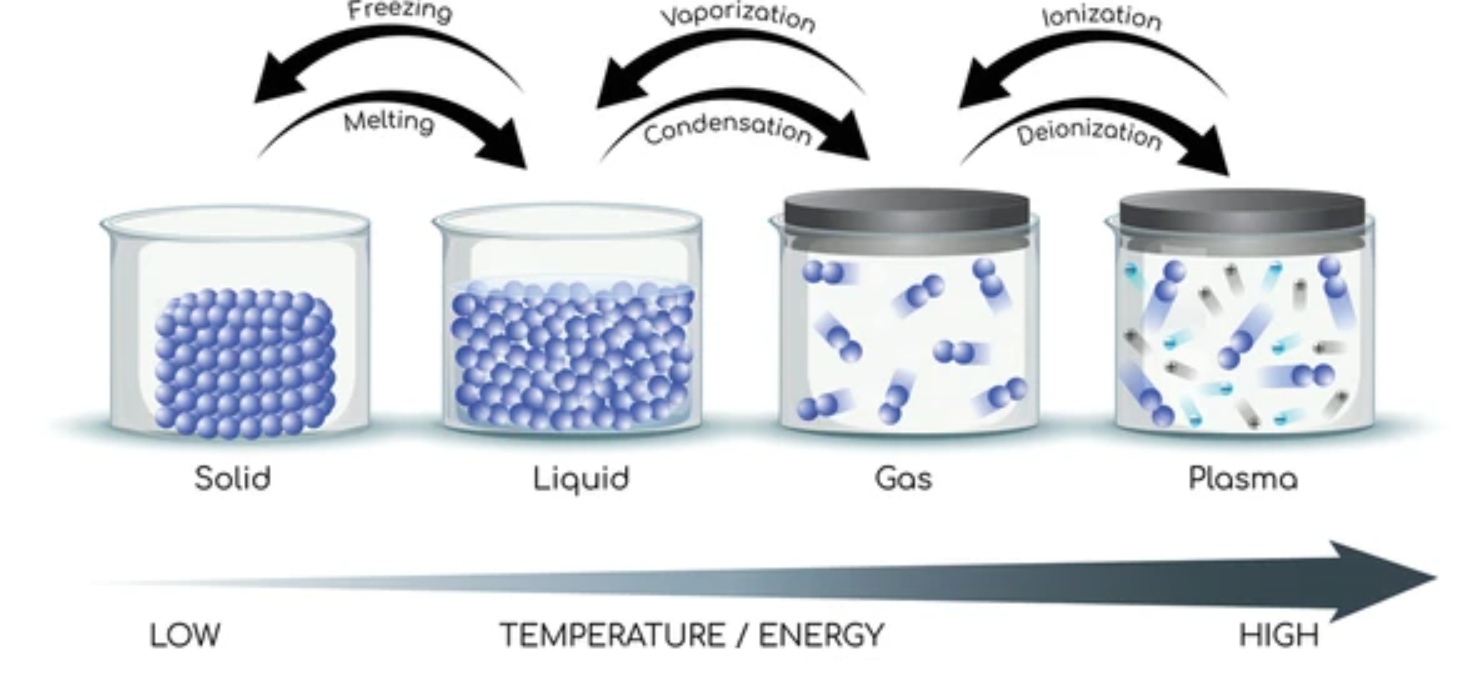
\includegraphics[width=0.85\linewidth]{pictures/matter_state}
	\end{center}
\end{frame}
% ===========================================================================

% ============================== Слайд ## ===================================
\begin{frame}{Відмінність властивостей плазми від властивостей нейтральних газів}{}
       \begin{enumerate}
       \item Взаємодія частинок плазми між собою характеризується кулонівськими силами притягнення та відштовхування, що зменшуються із відстанню більш повільно, ніж сили взаємодії нейтральних частинок.  Це означає, що взаємодія частинок у плазмі є не «парним», а «колективним» --- одночасно взаємодіють одна з одним велика кількість частинок.
       \item Електричні та магнітні поля сильно діють на плазму (у той же час як вони слабо діють на нейтральний газ), викликаючи появу у плазмі об’ємні заряди і струми та забезпечують ряд специфічних властивостей плазми.
       \end{enumerate}
\end{frame}
% ===========================================================================

% ============================== Слайд ## ===================================
\begin{frame}{Іонізація атома}{}
	\begin{onlyenv}<1>
		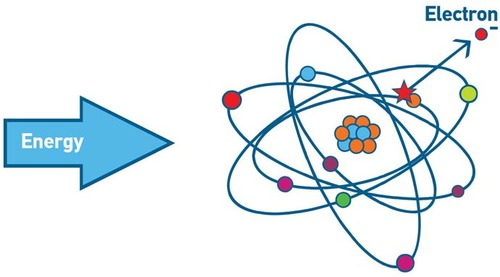
\includegraphics[width=1\linewidth]{ionization}
	\end{onlyenv}
	\begin{onlyenv}<2>
		\begin{block}{}
			Ступінь іонізації плазми характеризує відношення $\xi = n_i/n_0$.
			Рівняння Саха пов'язує ступінь іонізації $\xi$ з $n_0$ і $T$.
		\end{block}
		\begin{equation*}
			\frac{\xi^2}{1 - \xi} = n_0\frac{(2\pi m_e k T)^{3/2}}{h^3} \exp\left(-\frac{J}{kT}\right)
		\end{equation*}
		%---------------------------------------------------------
		\begin{mysidebyside}
			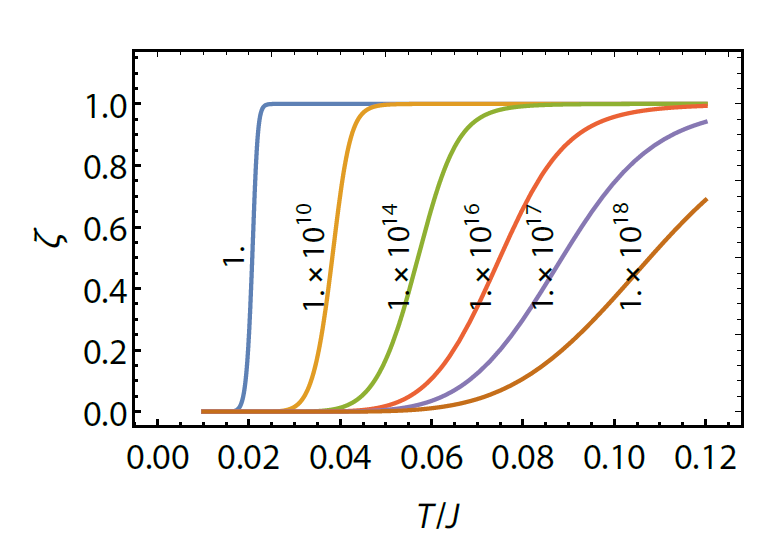
\includegraphics[width=1\linewidth]{xi_vs_T}
			\tcblower
			\small
			Ступінь іонізації термодинамічно рівноважної водневої плазми за різних значень густини плазми за різних значень густини, які зазначені на малюнку в одиницях см$^{−3}$.
		\end{mysidebyside}
		%---------------------------------------------------------
		Умовно прийнявши значення $\xi = \frac12 $ за точку переходу в іонізований стан.
	\end{onlyenv}
\end{frame}
% ===========================================================================

% ============================== Слайд ## ===================================
\begin{frame}{Температура плазми}{}
       \begin{alertblock}{}<1-2>
           Температура плазми у газорозрядних трубках сягає кількох еВ (десятки тисяч вольт). Чому лампи не плавляться?
       \end{alertblock}
       \begin{onlyenv}<2>
       При зіткненнях електронів з важкими іонами
       \begin{equation*}
           \frac{\Delta E}{E} \approx 4 \frac{m_e}{m_p} \approx 0.2 \%
       \end{equation*}

       \end{onlyenv}
       Електрон, що вдаряється об іон, відскакує від нього як тенісний м'яч від важкої вантажівки, майже не передаючи своєї енергії. Тому в досить широкій області температура електронів у плазмі $T_e$ відрізняється від температури іонів $T_i$.

      \begin{equation*}
          T_e \gg T_i.
      \end{equation*}

      \begin{block}{}\footnotesize\justifying
      За досить високої густини всяка плазма повинна швидко приходити в стан повної термодинамічної рівноваги термодинамічної рівноваги, в якому електронна та й іонна температури рівні.
      \end{block}
\end{frame}
% ===========================================================================

% ============================== Слайд ## ===================================
\begin{frame}{Види плазми}{}
	%---------------------------------------------------------
	\begin{onlyenv}<1>
		\begin{center}
			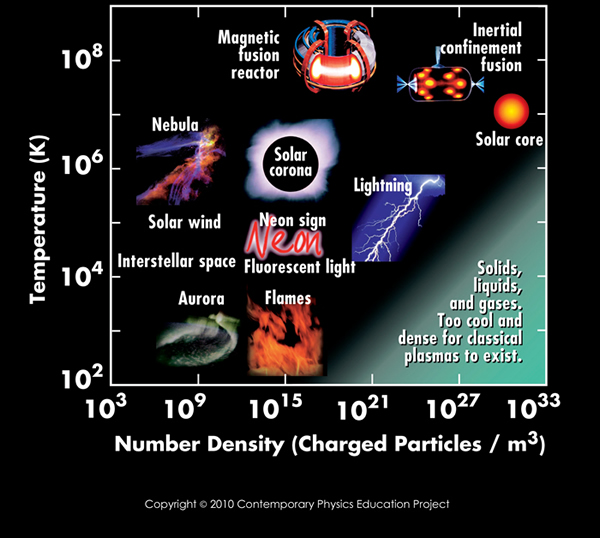
\includegraphics[width=0.75\linewidth]{plasma_properties}
		\end{center}
	\end{onlyenv}
	%---------------------------------------------------------
	\begin{onlyenv}<2>
		\begin{center}
			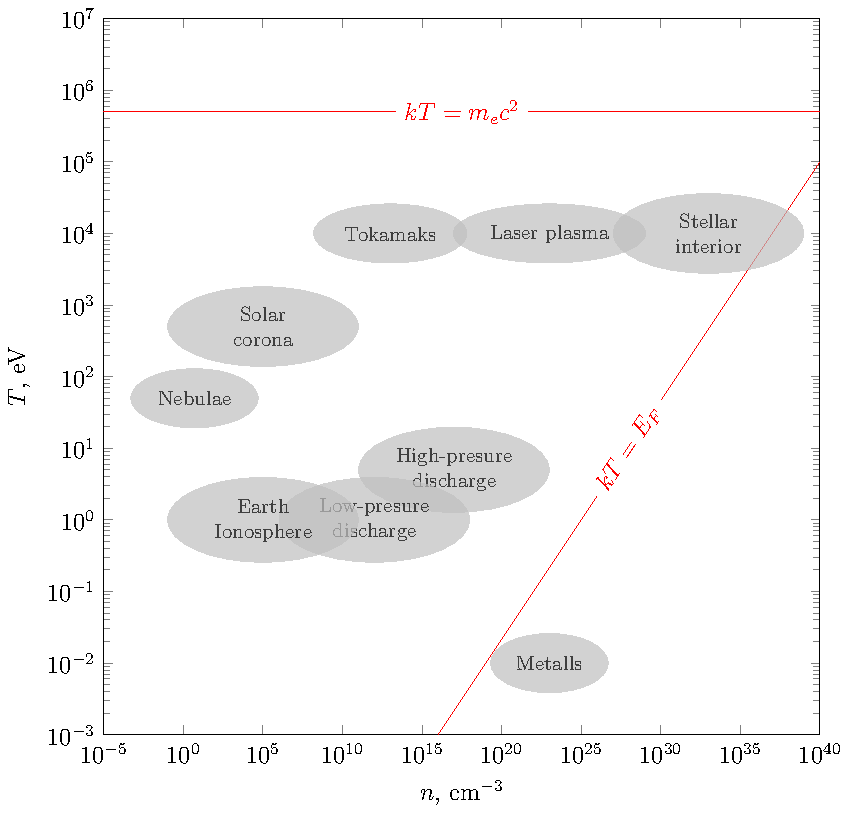
\includegraphics[width=0.75\linewidth]{plasma_types.pdf}
		\end{center}
	\end{onlyenv}
	%---------------------------------------------------------

    \begin{onlyenv}<3>
    \begin{table}[ht]\small
        \centering
        \begin{tabular}{lcc}
            \toprule
            Тип плазми & Концентрація (см$^{-3}$) & Температура (еВ) \\
            \midrule
            Метали             & $10^{24} \div 10^{25}$ & $ 0.01 $         \\
            Газовий розряд     & $10^{6} \div 10^{12}$  & $\sim 1$         \\
            Міжзоряна плазма   & $\sim 1 $              & $ 0.01 \div 1 $  \\
            Іоносфера Землі    & $ 10^2 \div 10^6 $     & $ 0.1  $  \\
            Сонячна атмосфера  & $ 10^{14} $            & $ \sim 1 $       \\
            Сонячне ядро       & $ 10^{25} $            & $ \sim 10^3 $     \\
            Токамак            & $ 10^{12}\div 10^{15}$ & $ \sim 10^3 $     \\
            \bottomrule
        \end{tabular}
    \end{table}
    \end{onlyenv}
\end{frame}
% ===========================================================================

% ============================== Слайд ## ===================================
\begin{frame}{Класифікація видів плазми}{}
       \begin{enumerate}
       \item Класична плазма плазма
       \begin{equation*}
           \frac{h^2 n^{2/3}}{m_e} \ll T \ll m_ec^2
       \end{equation*}
       \item Високотемпературна плазма:
       \begin{equation*}
           T \gg J
       \end{equation*}
       Низькотемпературна:
       \begin{equation*}
           T \ll  J
       \end{equation*}
       \item  Високотемпературна буває гарячою $\beta \sim 1$ і холодною $\beta \ll 1$:

       \begin{equation*}
           \beta = \frac{p_\text{г.-к.}}{p_m} = \frac{8\pi n k_\text{Б}T}{B^2}.
       \end{equation*}

       \end{enumerate}
\end{frame}
% ===========================================================================



\end{document}
